\documentclass{article}
\usepackage[UTF8]{ctex}
\usepackage{geometry}
\usepackage{multirow}
\usepackage{natbib}
\usepackage{float}
\geometry{left=3.18cm,right=3.18cm,top=2.54cm,bottom=2.54cm}
\usepackage{graphicx}
\pagestyle{plain}	
\usepackage{setspace}
\usepackage{enumerate}
\usepackage{caption2}
\usepackage{datetime} %日期
\renewcommand{\today}{\number\year 年 \number\month 月 \number\day 日}
\renewcommand{\captionlabelfont}{\small}
\renewcommand{\captionfont}{\small}
\begin{document}

\begin{figure}
    \centering
    
\includegraphics[width=8cm]{upc.png}

    \label{figupc}
\end{figure}

	\begin{center}
		\quad \\
		\quad \\
		\heiti \fontsize{45}{17} \quad \quad \quad 
		\vskip 1.5cm
		\heiti \zihao{2} 《计算科学导论》个人职业规划
	\end{center}
	\vskip 2.0cm
		
	\begin{quotation}
% 	\begin{center}
		\doublespacing
		
        \zihao{4}\par\setlength\parindent{7em}
		\quad 

		学生姓名:\underline{\qquad  李弟诚 \qquad \qquad}

		学\hspace{0.61cm} 号:\underline{\qquad 1907010105\qquad}
		
		专业班级:\underline{\qquad 计科1901 \qquad  }
		
        学\hspace{0.61cm} 院:\underline{计算机科学与技术学院}
% 	\end{center}
		\vskip 1.5cm
		\centering
		\begin{table}[h]
            \centering 
            \zihao{4}
            \begin{tabular}{|c|c|c|c|c|c|c|c|c|}
            % 这里的rl 与表格对应可以看到,姓名是r,右对齐的;学号是l,左对齐的;若想居中,使用c关键字。
                \hline
                \multicolumn{5}{|c|}{分项评价} &\multicolumn{2}{c|}{整体评价}  & 总    分 & 评 阅 教 师\\
                \hline
                自我 & 环境 & 职业 & 实施 & 评估与 & 完整性 & 可行性 &\multirow{2}*{} &\multirow{2}*{}\\
                分析& 分析& 定位 & 方案 & 调整 & 20\% & 20\% & ~&~ \\\            
                10\% & 10\% & 15\% & 15\% & 10\% & &  &~ &~\\
                \cline{1-7} 
                & & & & & & & ~&~ \\
                & & & & & & & ~&~ \\
                \hline      
            \end{tabular}
        \end{table}
		\vskip 2cm
		\today
	\end{quotation}

\thispagestyle{empty}
\newpage
\setcounter{page}{1}
% 在这之前是封面,在这之后是正文
\section{自我分析}

\subsection{自然条件}
我是一名16周岁的男生,身高172,身体健康,但眼镜度数不低,家住安徽省六安市。 \par
\subsection{性格分析}
我性格很开朗,并对很多事情很好奇。过去的我比较喜欢单打独斗,不是太擅长团队合作。不过进入大学以来,很多作业,任务,讨论的完成都离不开团队合作。这也使我渐渐喜欢上团队合作。\par
\subsection{教育与学习经历}
我与正常人一样,苦读了12年书来到大学接受进一步教育,曾经学过象棋,原先并没有接触过计算机相关知识。\par
\subsection{工作与社会阅历}
我没有工作经验。因为性格开朗,交往了许多朋友。跟着同学们出去旅游了2,3次。\par
\subsection{知识、技能与经验}
目前只掌握了一些c++与html的部分知识,并没有什么经验。\par
\subsection{兴趣爱好与特长}
本人目前对编程,算法和web前端开发有很浓厚的兴趣,并加入了ACM社团以接触更多的算法,还会在课余时间学习HTML并实践。而编程算是我的一项特长。\par
\section{环境分析}


\subsection{社会环境分析}\par
\subsubsection{政治形势}\par
我国政府为抵御国际经济环境对我国的不利影响,实行了 积极的财政政策和适度宽松的货币政策,出台了更加有力 的扩大内需措施,为产业发展创造良好机遇.。一些领域智 能系统的建设,为我国计算机产业和信息化的推广应用带 来新的发展机遇。而且党提出要大力推进信息化和工业化融合,加快推进电子信 息产业改造传统产业的步伐,为开拓工业计算机市场,创 造了新的巨大空间。 同时,计算机产业在国家相关政策的 支持下,仍将保持快速发展,特别是嵌入式系统计算机前 景看好,这为计算机产业的发展将带来良好机遇。
\subsubsection{经济形势}\par
当前经济形势对计算机业而言,其发展机遇主要表现在以下几个方面:
\begin{itemize}
		\item [1) ] 国际金融危机对于电子实力较强的大中型企业撼动力微弱,对计算机企业的冲击很小,人才、资本和市场都进一 步向大企业集中。在推动企业资本并购和产业整合迎来机 遇的同时,对大企业收购、整合优良资产、壮大实力、提 升竞争能力,将带来良好时机。 
		\item [2) ]基础产品价格下降,为企业盈利创造发展空间。 居民消 费能力将逐渐提升,特别是 3G 技术的商用、手机智能化、 新兴增值业务的出现以及国民经济的好转等,这些为电子 制造企业、计算机业的快速发展,起到了积极的推动作用。  
\end{itemize}
当前经济形势对计算机业而言,其面临的挑战主要表现在以下几个方面:
\begin{itemize} 
	\item [1) ]) 国际金融市场动荡和世界经济增长放缓,导致许多国家金 融市场出现了清偿危机,大公司缩减开支计划,减少并购 活动,全球对外直接投资流动性放缓。 
	\item [2) ] 产业深层次的矛盾仍制约着结构优化的快速发展。主要表 现在以下三个方面:一是企业低层次加工生产和产业链深 度发展的矛盾,二是企业核心技术的开发、掌握与产品结 构优化升级的矛盾,三是产业同质化与产业链整合的矛盾。 这些矛盾依然存在,并在一定程度上制约着产业结构优化.
	的快速发展。 
\end{itemize}
\subsubsection{就业形势}\par
近几年,IT 行业的迅速发展为计算机专业毕业生就业带来
了新的契机 ,但计算机专业毕业生就业形势仍然严峻。近年来,国
家人事部对大学应届毕业生的就业需求情况进行了调查分析,
尽管计算机、信息与电子类位列就业需求第二,但目前计算机专
业的学生数量已超过全国理工科大学生总数 1/3,随着毕业生数
量的急剧增加,计算机专业毕业生的就业竞争日趋激烈。同时,
计算机专业毕业生就业观过于理想化,同社会现实脱节,难以达
到应聘企业的人才需求。虽企业的岗位众多,但由于计算机专业
毕业生能力的参差不齐,所以造成了“企业用工荒,大学生就业
难”的局面,计算机专业大学生就业形势从而愈发严峻。
\subsection{家庭环境分析}
本人未婚,家庭小康。父母对我的期望,就是我能成为对别人来说不可或缺的人,能够有能力做出奉献的人。我们家族并没有什么特殊的传统,一切都很和谐。\par
\subsection{职业环境分析}
行业现状及发展趋势 我国网络技术发展迅速,企业对IT人才需求量不断增加,但高端IT人才严重匮乏。当今时代,电脑已经成为人们生活以及公司发展的必需品,所以现在电脑技术还是很有前途的,只要技术过硬,找到一份好工作,获得高额薪水,一切都不是问题。\par
就拿软件工程师来说,一般的职业要求如下:
\begin{itemize} 
	\item [1) ]计算机、软件、通信等相关专业本科及以上学历;

 	\item [2)]热爱编程,基础扎实,熟悉掌握但不限于JAVA/C++/Python/JS/HTML/GO等编程语言中的一种或数种,有良好的编程习惯;
	\item [3) ]具备独立工作能力和解决问题的能力、善于沟通,乐于合作,热衷新技术,善于总结分享,喜欢动手实践;   
	\item [4) ]对数据结构、算法有一定了解。
\end{itemize}
	
\par


\subsection{地域与人际环境分析}
我以后想去北京发展,北京的气候为典型的北温带半湿润大陆性季风气候,夏季高温多雨,冬季寒冷干燥,春、秋短促。\par
北京历史悠久,文化灿烂,是首批国家历史文化名城、中国四大古都之一和世界上拥有世界文化遗产数最多的城市,3060年的建城史孕育了故宫、天坛、八达岭长城、颐和园等众多名胜古迹。\par
北京还是一个互联网技术发展成熟的城市,许多大型IT企业也在北京,例如百度,新浪。在北京无论是就业还是创业都有着很好的机遇与地理优势。\par
想去北京发展的另一个原因,是因为我亲姐在北京大学就读,在我到北京发展后,一方面可以让家人之间互动更亲密,另一点就是我能依托我姐姐的人际发展我的人脉,这对我未来的发展尤为重要。我平日里相处的北京朋友也有一两个,可能在未来能帮助我建立良好的人脉关系。
\par
    \begin{figure}[H]
    	\centering
    	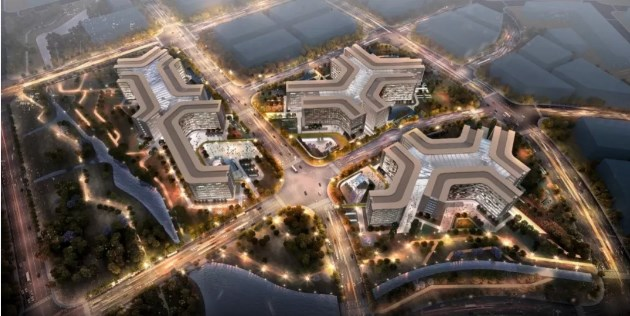
\includegraphics[width=8cm]{1.png}
    	\label{figupc}
    	  \caption{北京阿里总部} 
    \end{figure}
\section{职业定位}


\subsection{行业领域定位与理由}
我准备在IT行业就业。
身为一名计算机专业的学生,我自然要去与计算机关系最紧密的IT行业发光发热。IT行业不仅是一个待遇好,竞争公平,岗位多,视野开阔的行业,更是一个能把我在大学4年所学的知识落到实地的一个行业,也自然是我注定要去的一个行业。\par
 
\subsection{职业岗位起点定位与理由}
我要从一名软件工程师开始。理由如下:\par
我善于沟通,乐于合作,热衷新技术,喜欢动手实践,对用编程打开的新世界充满兴趣和向往。一直呆在ACM俱乐部里学习,相信毕业时我也能接触和掌握很多优秀的算法。目前我把HTML编程语言作为一项兴趣爱好,并与同班的高启东同学组队学习web前端开发,不断填补我的知识盲区。
我上网浏览了华为,阿里的校招信息,发现软件开发工程师 是众多职业中最适合我的一门,也是我最想工作的职业。\par
\subsection{职业目标与可行性分析}
\par 
\begin{enumerate}[(1)]
	\item短期目标
	\begin{itemize}
		\item 熟练掌握C++,python,html,css,javascript等语言。 
		\item 成功与同伴(高启东) 搭建一个校内跳蚤市场交易网络平台。
		\item 学习足量的算法与数据结构有关知识,开阔自己的视野。
		\item 能够成功组建一个小团队。
	\end{itemize}
	\item 长期目标
		\begin{itemize}
		\item 熟练应用自己所学的知识,并完成一些复杂的开发。
		\item 能够进入中产阶级,在公司里能够成为重要的软件开发人员。 
		\item 能够对自己所从事的行业有清晰的认识,并能准确预测该行业的未来发展形势。
		\item 能够成功组建一个大团队。
     	\end{itemize}
\end{enumerate}



\section{实施方案}

\begin{enumerate}[1、]
	\item 我可以借助大学这个广阔的平台,一方面可以在此期间多参加校内外编程比赛,增加自己的阅历,另一方面可以通过不断地向老师咨询来帮助自己认清眼前的路,在节约时间的同时保证了效率。自己性格外向,向往新知识,我会在大学这个人才汇聚的地方多结交志同道合的人,多实现一点小目标,为职业生涯目标奠定基础。
	\item 缺点和不足是每个人都会有的,在我看来,要想克服缺点,弥补不足,一方面要有毅力,另一方面就是要向这方面做的好的人看齐。我做事效率不高,便会留意身边做事效率高的同学,看看他们是怎么做到的。为了实现职业生涯目标,自然要多在课外多学习与自己职业相关的知识,一方面可以向经验丰富的老师们请教,另一方面可以在网上学习那些大牛们的学习路线。        
	\item    发展人际关系对自己的未来发展十分关键,以下几点是发展人际关系的关键:
		\begin{itemize}
	 、\item帮助他人成功。
	社交的本质就是不断用各种形式帮助其它人成功。共享出你的知识与资源、时间与精力、朋友与关系、同情与关爱,从而持续的为他人提供价值,同时提高自己的价值。
	\item努力让自己的付出多于回报。
	因为你会为别人提供价值,别人才会联系你。所以多考虑别人而不是自己。
	\item不要保留。
	不要以为友谊是有限的。这是投资,会越滚越多。            
	\item了解你交往的人。
	对于自己身边的人,自己应该对他们有足够的了解,这样才能找到彼此身上的共同点,建立更深的联系。         如何处理人际关系和发展人脉以实现职业生涯目标。
		\end{itemize}
	\item 
	工作和家庭,生活是相辅相成的个体,而不是矛盾体。要想能够专心致志地工作,必须处理好家庭和生活中的问题。将父母接到自己工作的城市或者常回家看看,保证家庭的和睦,也就保证了生活的幸福。人工作是为了家庭,规划好用在家庭生活与用在工作上的时间与精力,才能使两者协调发展,相辅相成。
	
	\item 
	在自己的职业生涯中保持一颗乐观的心是关键,我将来的职业绝不会轻松,更应该保持乐观,防止被工作压垮。当然,仅仅靠一颗乐观强大的心可能并不够。科学证明,运动是保持身心健康,舒缓压力的好方法。多与朋友到户外健身,不定期远足或者在书中获得心灵寄托都是我认为不错的释放工作压力,保证身心健康的方法,也更有利于我们实现职业生涯目标。
	如何处理释放工作压力、保证身心健康以实现职业生涯目标。
\end{enumerate}
\par

\section{评估与调整}

\subsection{评估时间}
我今后每学期都会按照自己的职业发展规划对自己进行评估。\par
\subsection{评估内容}
学分绩,自己搭建网站的经济效益、访问量,掌握编程语言的数量和掌握程度。
\par
\subsection{调整原则}
应考虑与自身情况的匹配性、与环境的适应性、操作实施的可行性等。\par

\bibliographystyle{plain}
\bibliography{references}


\end{document}
